\begin{task}
\TT{Wyznacz współczynniki zespolonego szeregu Fouriera dla okresowego sygnału $f(t)$ przedstawionego na rysunku. Wykorzystaj więdzę o liniowości szeregu Fouriera i o wpływie przesunięcia sygnału w czasie na współczynniki szeregu Fouriera.}{Calculate coefficients of the periodic signal $f(t)$ shown below for the expansion into a complex exponential Fourier series. Use knowledge about linearity of complex exponential Fourier series and about the effect of signal shift in time on the complex exponential Fourier series.}

\begin{figure}[H]
    \centering
    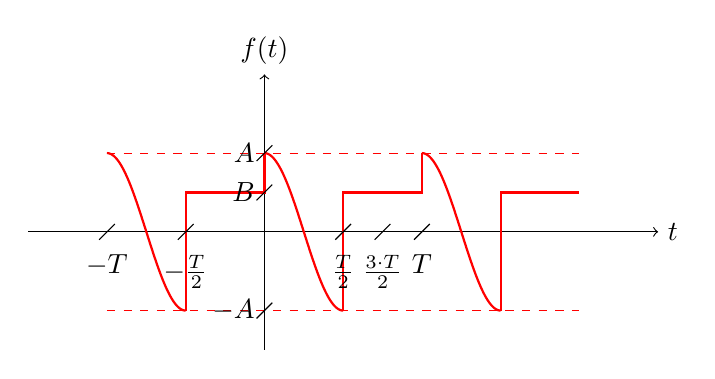
\begin{tikzpicture}
    %\draw (0,0) circle (1in);
    \draw[->] (-3.0,+0.0) -- (+5.0,+0.0) node[right] {$t$};
    \draw[->] (+0.0,-1.5) -- (+0.0,+2.0) node[above] {$f(t)$};
    \draw[scale=1.0,domain=-2.0:-1.0,samples=100,smooth,variable=\x,red,thick] plot ({\x},{0.0+1*cos(\x*180.0/3.141592*1*3.141592/1.0)});
    \draw[-,red, thick] (-1.0,-1.0) -- (-1.0,0.5) -- (0.0,0.5) -- (0.0,1.0);
    \draw[scale=1.0,domain=0.0:1.0,samples=100,smooth,variable=\x,red,thick] plot ({\x},{0.0+1*cos(\x*180.0/3.141592*1*3.141592/1.0)});
    \draw[-,red, thick] (1.0, -1.0) -- (1.0,0.5) -- (2.0,0.5) -- (2.0,1.0);
    \draw[scale=1.0,domain=2.0:3.0,samples=100,smooth,variable=\x,red,thick] plot ({\x},{0.0+1*cos(\x*180.0/3.141592*1*3.141592/1.0)});
    \draw[-,red, thick] (3.0, -1.0) -- (3.0,0.5) -- (4.0,0.5);

    \draw[-,red, dashed] (-2.0,1.0) -- (4.0,1.0);
    \draw[-,red, dashed] (-2.0,-1.0) -- (4.0,-1.0);
    %\draw[-] (-1.0-0.1,-0.1)--(-1.0+0.1,0.1) node[midway, below, outer sep=10pt,align=center] {$-\frac{T}{2}$};
    \draw[-] (-2.0-0.1,-0.1)--(-2.0+0.1,0.1) node[midway, below, outer sep=5pt] {$-T$};
    \draw[-] (-1.0-0.1,-0.1)--(-1.0+0.1,0.1) node[midway, below, outer sep=5pt] {$-\frac{T}{2}$};
    \draw[-] (+1.0-0.1,-0.1)--(+1.0+0.1,0.1) node[midway, below, outer sep=5pt] {$\frac{T}{2}$};
    \draw[-] (+2.0-0.1,-0.1)--(+2.0+0.1,0.1) node[midway, below, outer sep=5pt] {$T$};
    \draw[-] (+1.5-0.1,-0.1)--(+1.5+0.1,0.1) node[midway, below, outer sep=5pt] {$\frac{3 \cdot T}{2}$};
    \draw[-] (-0.1,+0.5-0.1)--(+0.1,+0.5+0.1) node[midway, left] {$B$};
    \draw[-] (-0.1,+1.0-0.1)--(+0.1,+1.0+0.1) node[midway, left] {$A$};
    \draw[-] (-0.1,-1.0-0.1)--(+0.1,-1.0+0.1) node[midway, left] {$-A$};
    
    \end{tikzpicture}
\end{figure}

\TT{W pierwszej kolejności należy opisać sygnał za pomocą wzoru.}{Periodic signal $f(t)$, as a piecewise function, is given by:}

\begin{equation}
f(t)=\begin{cases}A \cdot cos\left( \frac{2\pi}{T} \cdot t\right) & t \in \left ( 0+k \cdot T; \frac{T}{2}+k \cdot T \right ) \\
B & t \in \left ( \frac{T}{2}+k \cdot T; T+k \cdot T \right )\end{cases} \wedge k \in \TT{C}{Z}
\end{equation}

\TT{Jeśli przyjrzeć się dokładniej sygnałowi $f(t)$, można zauważyć, że składa się on z sygnałów $g(t)$ i $h(t)$, dla których już wcześniej obliczyliśmy współczynniki zesolonego szeregu Fourira.}{If we look carefully, signal $f(t)$ may be decomposed into two signals $g(t)$ and $h(t)$ for which we have already calculated Fourier series coefficients. The signals are given below:}

\begin{figure}[H]
    \centering
    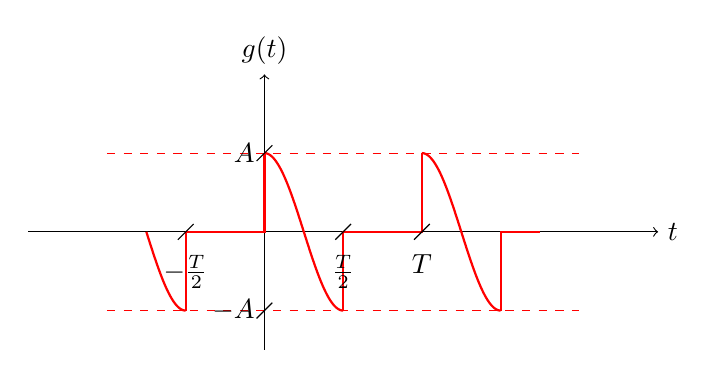
\begin{tikzpicture}
    %\draw (0,0) circle (1in);
    \draw[->] (-3.0,+0.0) -- (+5.0,+0.0) node[right] {$t$};
    \draw[->] (+0.0,-1.5) -- (+0.0,+2.0) node[above] {$g(t)$};
    \draw[scale=1.0,domain=-1.5:-1.0,samples=100,smooth,variable=\x,red,thick] plot ({\x},{0.0+1*cos(\x*180.0/3.141592*1*3.141592/1.0)});
    \draw[-,red, thick] (-1.0,-1.0) -- (-1.0,0.0) -- (0.0,0.0) -- (0.0,1.0);
    \draw[scale=1.0,domain=0.0:1.0,samples=100,smooth,variable=\x,red,thick] plot ({\x},{0.0+1*cos(\x*180.0/3.141592*1*3.141592/1.0)});
    \draw[-,red, thick] (1.0, -1.0) -- (1.0,0.0) -- (2.0,0.0) -- (2.0,1.0);
    \draw[scale=1.0,domain=2.0:3.0,samples=100,smooth,variable=\x,red,thick] plot ({\x},{0.0+1*cos(\x*180.0/3.141592*1*3.141592/1.0)});
    \draw[-,red, thick] (3.0,-1.0) -- (3.0,0.0) -- (3.5,0.0);
    \draw[-,red, dashed] (-2.0,1.0) -- (4.0,1.0);
    \draw[-,red, dashed] (-2.0,-1.0) -- (4.0,-1.0);
    %\draw[-] (-1.0-0.1,-0.1)--(-1.0+0.1,0.1) node[midway, below, outer sep=10pt,align=center] {$-\frac{T}{2}$};
    \draw[-] (-1.0-0.1,-0.1)--(-1.0+0.1,0.1) node[midway, below, outer sep=5pt] {$-\frac{T}{2}$};
    \draw[-] (+1.0-0.1,-0.1)--(+1.0+0.1,0.1) node[midway, below, outer sep=5pt] {$\frac{T}{2}$};
    \draw[-] (+2.0-0.1,-0.1)--(+2.0+0.1,0.1) node[midway, below, outer sep=5pt] {$T$};
    \draw[-] (-0.1,+1.0-0.1)--(+0.1,+1.0+0.1) node[midway, left] {$A$};
    \draw[-] (-0.1,-1.0-0.1)--(+0.1,-1.0+0.1) node[midway, left] {$-A$};
    
    \end{tikzpicture}
\end{figure}

\begin{figure}[H]
\centering
\begin{tikzpicture}
  %\draw (0,0) circle (1in);
  \draw[->] (-3.0,+0.0) -- (+5.0,+0.0) node[right] {$t$};
  \draw[->] (+0.0,-1.5) -- (+0.0,+1.5) node[above] {$h(t)$};
  \draw[-,red, thick] (-2.5,+0.0) -- (-2.0,+0.0) -- (-2.0,+1.0) -- (-1.0,+1.0) -- (-1.0,+0.0)--(+0.0,+0.0) -- (+0.0,+1.0) -- (+1.0,+1.0) -- (+1.0,+0.0) -- (+2.0,+0.0) -- (+2.0,+1.0) -- (3.0,1.0) -- (3.0,0.0) -- (3.5,0.0);
  %\draw[-] (-1.0-0.1,-0.1)--(-1.0+0.1,0.1) node[midway, below, outer sep=10pt,align=center] {$-\frac{T}{2}$};
  \draw[-] (-1.0-0.1,-0.1)--(-1.0+0.1,0.1) node[midway, below, outer sep=5pt,align=center] {$-\frac{T}{2}$};
  \draw[-] (+1.0-0.1,-0.1)--(+1.0+0.1,0.1) node[midway, below, outer sep=5pt] {$\frac{T}{2}$};
  \draw[-] (+2.0-0.1,-0.1)--(+2.0+0.1,0.1) node[midway, below, outer sep=5pt] {$T$};
  \draw[-] (-0.1,1.0-0.1)--(+0.1,1.0+0.1) node[midway, left] {$B$};
\end{tikzpicture}
\end{figure}

\TT{Dokładnie rzecz ujmując, sygnał $f(t)$ jest sumą sygnałów: $g(t)$ i $h(t)$ przesuniętego w czasie o pół okresu ($\frac{T}{2}$):}{To be precise, the $f(t)$ signal will be the sum of $g(t)$ and $h(t)$ shifted in time by $\frac{T}{2}$:}

\begin{equation}
f(t)=g(t) + h\left(t-\frac{T}{2}\right)
\end{equation}

\TT{Wykorzystując więdzę o liniowości szeregu Fouriera i o wpływie przesunięcia sygnału w czasie na współczynniki szeregu Fouriera możemy napisać, że:}{Based on linearity of complex exponential Fourier series and about the effect of signal shift in time on the complex exponential Fourier series, we can write:}

\begin{align*}
F_k&=G_k+H_k \cdot e^{-\jmath \cdot k \cdot \frac{2\pi}{T} \cdot \frac{T}{2}}\\
F_k&=G_k+H_k \cdot e^{-\jmath \cdot k \cdot \pi}\\
F_k&=G_k+H_k \cdot (-1)^k\\
\end{align*}

\TT{Na podstawie wcześniej obliczonych zadań, współczynniki zespolonego szeregu Fouriera dla sygnałów $g(t)$ i $h(t)$ wynoszą odpowiednio:}{From previous tasks we know, that coefficients for the expansion into a complex exponential Fourier series of $g(t)$ and $h(t)$ signals are equal to:}

\begin{align*}
G_0&=0\\
G_1&=\frac{A}{4}\\
G_{-1}&=\frac{A}{4}\\
G_k&=\jmath \cdot \frac{A \cdot k}{2\pi} \cdot \left( \frac{ (-1)^{k}  + 1}{1 -k^2} \right)\\
\end{align*}

\begin{align*}
H_0&=\frac{B}{2}\\
H_k&=\jmath \cdot \frac{B}{k\cdot 2 \pi}\cdot \left( (-1)^{k} -1 \right)\\
\end{align*}

\TT{Teraz możemy wyznaczyć współczynniki dla sygnału $f(t)$:}{Right now we know everything to calculate $F_k$ coefficients:}

\begin{align*}
F_k&=G_k+H_k \cdot (-1)^k = \\
&= \jmath \cdot \frac{A \cdot k}{2\pi} \cdot \left( \frac{ (-1)^{k}  + 1}{1 -k^2} \right) + \jmath \cdot \frac{B}{k\cdot 2 \pi}\cdot \left( (-1)^{k} -1 \right) \cdot (-1)^k=\\
&= \jmath \cdot \left[\frac{A \cdot k}{2\pi} \cdot \left( \frac{ (-1)^{k}  + 1}{1 -k^2} \right) + \frac{B}{k\cdot 2 \pi}\cdot \left( 1 - (-1)^{k}\right)\right]
\end{align*}

\TT{Podobnie dla współczynnika $F_0$}{}

\begin{align*}
F_0&=G_0 + H_0 \cdot (-1)^0=\\
 &= 0 + \frac{B}{2} \cdot 1=\\
 &= \frac{B}{2}
\end{align*}

\TT{Podobnie dla współczynnika $F_1$ i $F_{-1}$}{}

\begin{align*}
F_1&=G_1 + H_1 \cdot (-1)^1 =\\
&= \frac{A}{4} + \jmath \cdot \frac{B}{1\cdot 2 \pi}\cdot \left( (-1)^{1} -1 \right) \cdot (-1) =\\
&= \frac{A}{4} + \jmath \cdot \frac{B}{\pi}
\end{align*}

\begin{align*}
F_{-1}&= G_{-1} + H_{-1}\cdot (-1)^{-1} =\\
&= \frac{A}{4} + \jmath \cdot \frac{B}{(-1)\cdot 2 \pi}\cdot \left( (-1)^{-1} -1 \right) \cdot (-1) =\\
&= \frac{A}{4} - \jmath \cdot \frac{B}{\pi}
\end{align*}

\TT{Ostatecznie współczynniki zespolonego szeregu Fouriera dla sygnału $f(t)$ wynoszą}{}

\begin{align*}
F_0&=\frac{B}{2}\\
F_1&=\frac{A}{4} + \jmath \cdot \frac{B}{\pi}\\
F_{-1}&=\frac{A}{4} - \jmath \cdot \frac{B}{\pi}\\
F_k&= \jmath \cdot \left[\frac{A \cdot k}{2\pi} \cdot \left( \frac{ (-1)^{k}  + 1}{1 -k^2} \right) + \frac{B}{k\cdot 2 \pi}\cdot \left( 1 - (-1)^{k}\right)\right]
\end{align*}

\end{task}